% Created 2021-04-17 Sat 11:25
% Intended LaTeX compiler: pdflatex
\documentclass[11pt]{article}
\usepackage[utf8]{inputenc}
\usepackage[T1]{fontenc}
\usepackage{graphicx}
\usepackage{grffile}
\usepackage{longtable}
\usepackage{wrapfig}
\usepackage{rotating}
\usepackage[normalem]{ulem}
\usepackage{amsmath}
\usepackage{textcomp}
\usepackage{amssymb}
\usepackage{capt-of}
\usepackage{hyperref}
\author{Laurent Lejeune}
\date{\today}
\title{Mojo Fertility Assignment}
\hypersetup{
 pdfauthor={Laurent Lejeune},
 pdftitle={Mojo Fertility Assignment},
 pdfkeywords={},
 pdfsubject={},
 pdfcreator={Emacs 26.3 (Org mode 9.4)}, 
 pdflang={English}}
\begin{document}

\maketitle

\section{Context and Goal}
\label{sec:org466e312}

In the context of sperm quality assessment, we devise an algorithm that counts the number of spermatozoa
on image-slices obtained through a camera.


\section{Method}
\label{sec:orgdd813ff}

Our solution relies on a Random Forest classifier trained on patches.
In a nutshell, we first leverage the \href{https://www.epfl.ch/labs/cvlab/software/descriptors-and-keypoints/daisy/}{DAISY} descriptors to characterize local regions.
We then devise a sampling strategy to augment the scarce positive set, while a hard negative mining strategy allows to select relevant samples from the redundant and ambiguous
negative set.

The main challenges of this problem lies in (1) the strong imbalance of the provided annotated dataset, where the mean number of positive samples per image is around \(10\), and (2) the fact that many spermatozoa that are not
in focus must be classified as negative.

It is therefore clear that training an efficient classifier in this context requires an appropriate
negative mining strategy, since a vast amount of potential negative patches carry no relevant information, e.g.
homogeneous taint, or obvious artifacts (debris), while many negative samples (out of focus) are visually similar to
positives.

We now describe in more details our pipeline.
After introducing some notations, we describe our feature extraction instance, follow with
our negative mining strategy, and finish by giving details on the setting of hyper-parameters using K-fold cross-validation.


\subsection{Notations}
\label{sec:orgc77ef82}

\begin{itemize}
\item \(\bm{X} \in \mathbb{R}^{N \times D}\) a feature matrix where rows are samples and columns
are the components of the feature vector.
\item \(\bm{Y} \in \{0;1\}^N\) the ground-truth label vector of the corresponding samples
\item \(\hat{y}= f_{\theta}(x): \mathbb{R}^{D} \rightarrow [0;1]\) is a classifier that outputs the probability of an input vector to be an object of interest.
\end{itemize}

\subsection{Feature extraction}
\label{sec:org934fb94}

DAISY descriptors have been proposed as an improvement over the popular \href{https://en.wikipedia.org/wiki/Scale-invariant\_feature\_transform}{Scale Invariant Feature Transform (SIFT)}.
In particular, it is devised to compute dense descriptors (one per pixel) using a fast algorithm.

In our scenario, we do not need to localize samples precisely.
We therefore prefer to extract descriptors with a decimation step of \(8\), so as to save memory.
For an image of size \(1920 \times 1200\), we obtain a total of \(9000\) descriptors encoded in \href{https://en.wikipedia.org/wiki/Half-precision\_floating-point\_format}{Half-precision floating-point format}.

The \href{https://github.com/scikit-image/scikit-image/blob/main/skimage/feature/\_daisy.py\#L9-L222}{algorithm} computes dense descriptors in \(\sim 5\) seconds per image, making \(\sim 50\) minutes for the full dataset (500 images).

\subsection{Classifier}
\label{sec:org0f61b03}

To classify patches, we use a \href{https://en.wikipedia.org/wiki/Random\_forest}{Random Forest} classifier.
We set \(T=100\) trees, \(D'=\sqrt{D}\) randomly picked feature component per split, and stop growing a tree
when all leaves contain less than \(N'=0.05 \cdot (2 \cdot N_p)\) samples.
As purity criterion, we select the \href{https://en.wikipedia.org/wiki/Gini\_coefficient}{Gini} index.

\subsection{Augmentation of positives}
\label{sec:orgf6647b5}

To alleviate the lack of positives, we define a circular region centered on a \((x,y)\) location
annotated as positive, and
take as positive patches all patches whose center is in a close vicinity.
In particular, we compute a pairwise distance matrix between all positives and all other samples,
threshold the values of this matrix by a pre-defined constant \(L_2\) -norm,
and augment our positive set with the corresponding samples.

\subsection{Hard negative mining}
\label{sec:org6b3f574}

We follow a simple iterative strategy to identify ``hard'' negatives.
Our idea is to pick relevant negative samples by using the predicted probability of the model itself.

Let \(\mathcal{S}_p\) the set of positive samples, obtained as in Sec. \ref{sec:orgf6647b5}, such that \(|\mathcal{S}_p|=N_p\).
Also, let \(\mathcal{S}_n\) the set of negative samples, such that \(|\mathcal{S}_n|=N_n \gg N_p\).

Our algorithm runs as follows:

\begin{enumerate}
\item Train \(f_\theta\) by fitting \(T\) trees using positive set \(\mathcal{S}_p\), and negative set \(\mathcal{S}'_n\) with \(N_p\)
samples chosen by uniform random sampling from \(\mathcal{S}_n\).
\item Predict probability of samples from \(\mathcal{S}_n\) using \(f_\theta\) to get \(\hat{y}^-\)
\item Sort \(\mathcal{S}_n\) according to \(\hat{y}^-\) in descending order, and set
\(\mathcal{S}'_n\) with the first \(N_p\) elements of \(\mathcal{S}_n\).
\item Train \(f_\theta\) by fitting \(T\) \textbf{additional trees} using \(\mathcal{S}_p\) and \(\mathcal{S}'_n\).
\item Repeat steps 2-4 \(M\) times.

Fig. \ref{fig:org08d1214} illustrates our sampling strategy on an example image.

\begin{figure}[htbp]
\centering
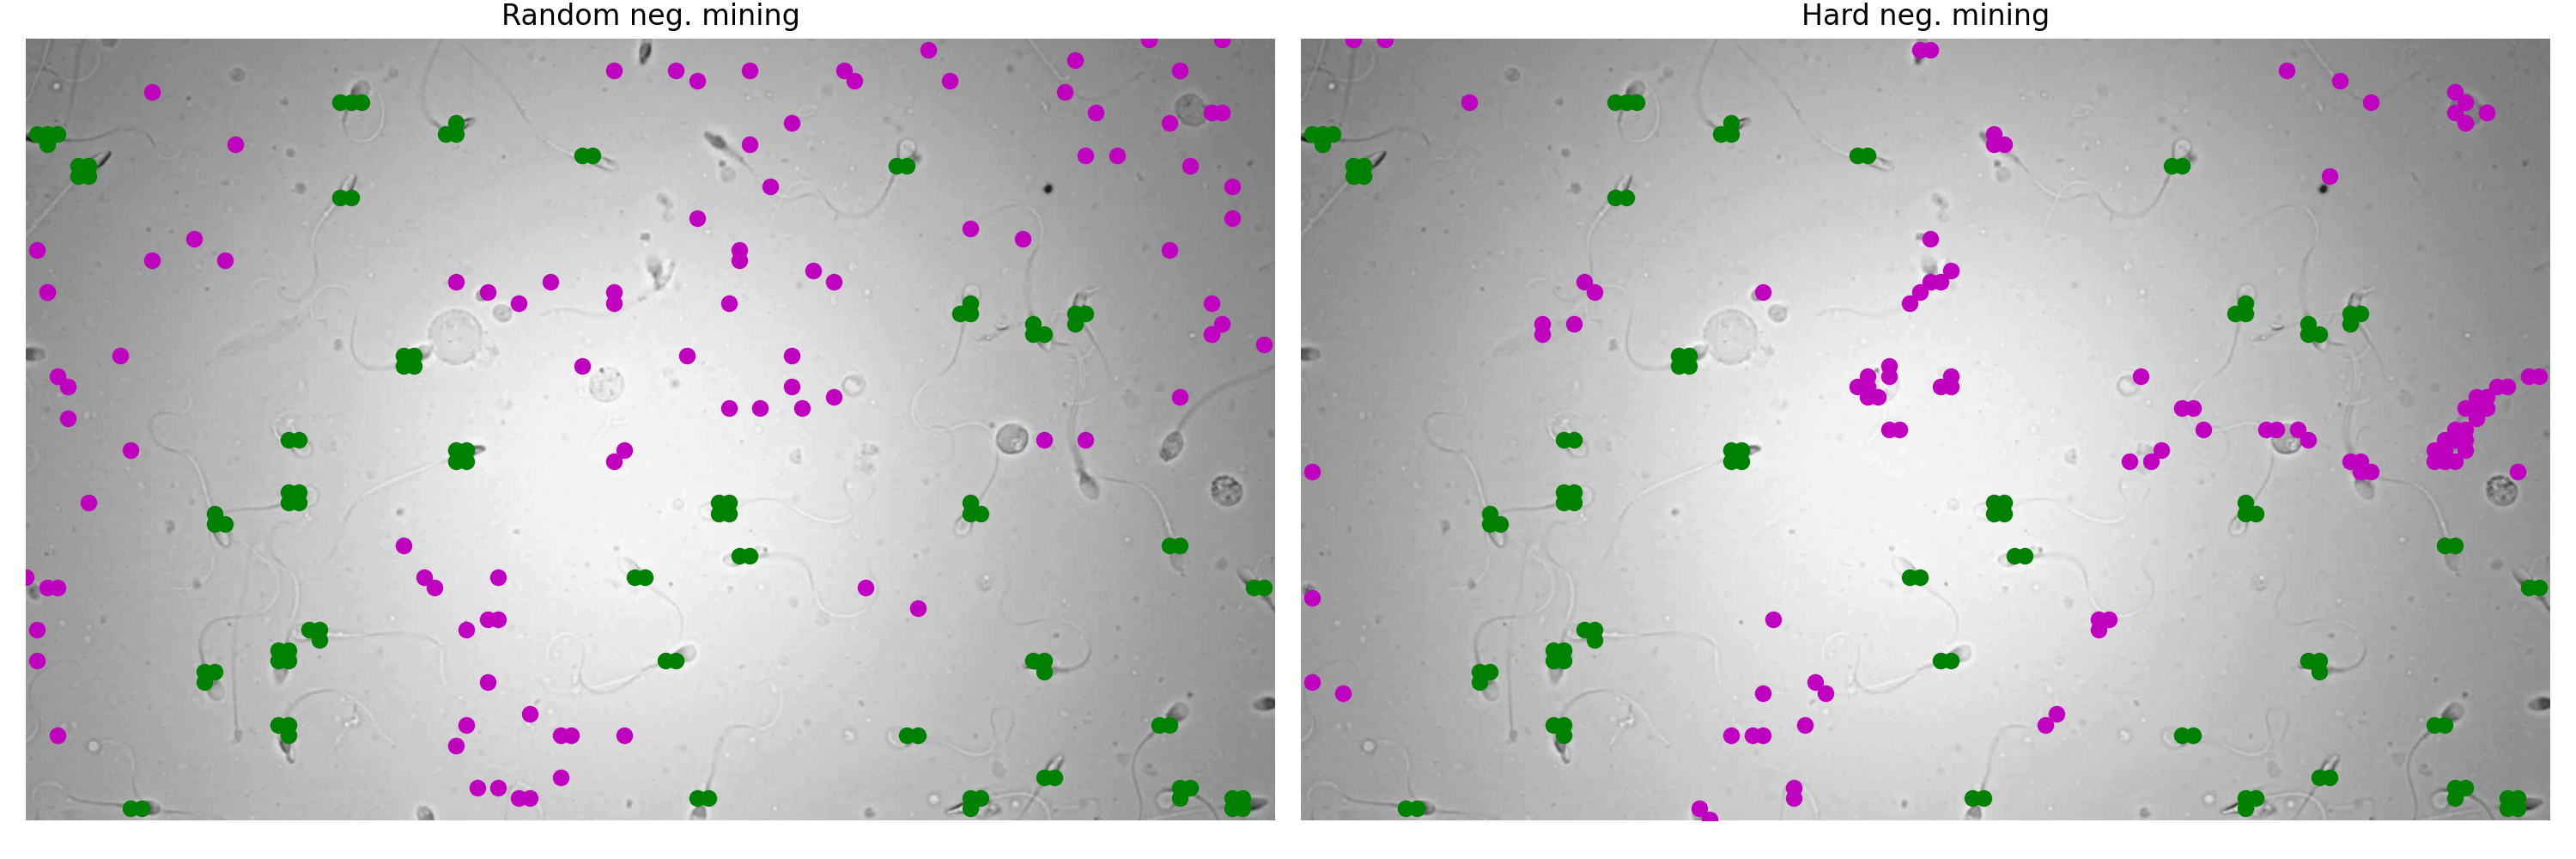
\includegraphics[width=.9\linewidth]{../results/hard_mining/mining_prev.png}
\caption{\label{fig:org08d1214}Sample mining strategy on an image. Positives are in green, negatives are in magenta. Left: For the first iteration, negatives are sampled at random. Right: Negatives are sampled according to our hard mining strategy after \(4\) iterations.}
\end{figure}
\end{enumerate}

\subsection{Tuning of hyper-parameters}
\label{sec:org8d9bd5e}

Recall that our task is to \textbf{count} the number of spermatozoa.
Since our pipeline extracts \(\sim 9000\) samples per image, we need a criteria to select among these the
candidates that are more likely to be positives.

In particular, we look for a threshold \(\tau\) on the output probabilities \(\hat{y}\)
using a 4-fold cross-validation strategy.
We let aside a subset of \(50\) images for the testing phase, and divide the remaining \(450\)
images in 4 non-overlapping validation subsets of equal size (\(125\) images), while
the training set of a fold contains all other samples.

Fig. \ref{fig:orgd59f3c4} shows the absolute count error on the validation set using the hard negative mining strategy
for increasing values of \(\tau\).
We select the optimal value \(\tau^*\) that minimizes the error.

\begin{figure}[htbp]
\centering
\includegraphics[width=.9\linewidth]{../results/hard_mining/cross_validation.png}
\caption{\label{fig:orgd59f3c4}Absolute count error with respect to threshold \(\tau\) using our hard negative mining strategy. We show the mean absolute count error over 4 folds, with dashed line representing standard deviation.}
\end{figure}

\section{Experiments}
\label{sec:org852a0e8}

So as to prove the relevance of our hard mining strategy, we perform an ablation study.
In particular, we introduce classification methods:

\begin{itemize}
\item \textbf{Hard Negative Mining Random Forest}: A Random Forest classifiers containing \(M \cdot T\) trees
optimized using an augmented positive set (Sec. \ref{sec:orgf6647b5} ), and the proposed hard negative mining strategy (Sec. \ref{sec:org6b3f574}).
\item \textbf{Random Negative Mining Random Forest}: A Random Forest classifiers containing \(M \cdot T\) trees
optimized using the same augmented positive set, and randomly sampled negatives.
\end{itemize}

Both methods are cross-validated (as in Sec. \ref{sec:org8d9bd5e}) using the same training and validation subsets to get their respective
optimal threshold value \(\tau^*\).

We then re-train both methods on an identical data subset (union of training and validation set used in Sec. \ref{sec:org8d9bd5e}), and compute performance metrics on the remaining set (test set).

Letting \(C\) and \(\hat{C}\) the true and estimated counts, respectively, we report the following metrics:

\begin{itemize}
\item \(\Delta = |\hat{C} - C|\): The absolute estimated error.
\item \(\bar{\Delta} = \frac{|\hat{C} - C|}{C}\): The normalized estimated count.
\end{itemize}
\end{document}
